We now analyze the greedy algorithm and prove that it recolors at most 
$\frac{3}{2} \cdot k$ vertices, 
where $k$ is the minimum number of vertices that must be recolored to achieve a convex
coloring.
%
We also show that the analysis is tight even in trees.
%
For the special case when $G$ is a simple path, 
we show that the greedy algorithm achieves a $\frac{5}{4}$ approximation ratio.
We show that the analysis is tight for this special case as well.

Recall that $D$ is the set of disconnected pairs in $G$, 
$I \subseteq D$ is the set of independent paths colored by the greedy algorithm, 
and let $I^* \subseteq D$ be the set of independent paths colored by an arbitrary, 
but fixed,
optimal path-recoloring.  
%
Define $\alpha := \frac{|I^*|}{|I|}$,
then by Lemma~\ref{lm:cost} the ratio between the number of 
vertices recolored by the greedy algorithm and the number of vertices
recolored by an optimal path-recoloring is:
\[
r := \frac{|D| - |I|}{|D| - |I^*|}
= \frac{|D| - |I|}{|D| - \alpha |I|}
\]
We now analyze the relationship between $|I|$, $|D|$ and $\alpha$.

Let $\ell_p$ be the number of vertices on a path $p$, and observe that:

\begin{lemma}
\label{lemma:assign}
If $p' \in I^* \setminus I$ then there is a path $p \in I$ that is in
conflict with $p'$, and $\ell_p \leq \ell_{p'}$.
\end{lemma}
\begin{proof}
Consider the running of the greedy algorithm at the most recent point,
where $I$ contains no path with a distance greater than $\ell_{p'}$.  If,
at this point, there is no path in $I$ that is in conflict with $p'$
then nothing prevents the greedy algorithm from adding $p'$ to $I$.
\qed{}\end{proof}

Next, we assign each optimal path to a greedy path.
%
Given a path $p' \in I^*$, the \emph{conflict source} of $p'$ is $p'$
itself if $p' \in I$, otherwise it is an arbitrary shortest path in
$I$ that is in conflict with $p'$.
%
Notice that this is a many-to-one assignment, that is, several optimal
paths can be assigned to a single greedy path.
%
For a path $p \in I$, the set of paths in $I^*$ such that $p$ is their
conflict source is denoted as $N(p)$.  The members of $N(p)$ are
called the \emph{neighbours} of $p$.

Due to Lemma~\ref{lemma:assign} we have that:

\begin{observation}
\label{co:dpLeqDp'}
For every path $p \in I$, if $p' \in N(p)$, then $\ell_p \leq \ell_{p'}$.
\end{observation}

Denote $d_p := |N(p)|$ and refer to $d_p$ as the \emph{degree} of $p$.
Our next goal is to find an upper bound to $d_p$, for $p \in I$.

\begin{lemma}
\label{lm:num_in_conflict}
$d_p \leq \ell_p - 1$.
\end{lemma}
\begin{proof}
Given a path $p \in I$, we show that the number of paths in $I^*$ that
are in conflict with $p$ is at most $\ell_p - 1$.
%
Associate a vertex in $p$ to every path that is in conflict with $p$.
For a path that is in direct conflict with $p$ associate a common
vertex of these paths, for a path that is in indirect conflict due to
color $c$, associate the vertex that has color $c$ in $p$.  Recall
that no two paths in $I^*$ are in conflict, and observe that
associating the same vertex to more than one path implies the
existence of such conflict. 
Finally, only one end point of $p$ can be associated with a path in $I^*$, 
or otherwise, $I^*$ is not independent.
\qed{}\end{proof}

In what follows we obtain two lower bounds on $|D|$, which translate
into two upper bounds on the approximation ratio $r$.

\begin{lemma}
\label{lemma:kernel}
$|D| \geq 2|I^*|$.
\end{lemma}
\begin{proof}
Every path in $I^*$ has length of at least 3, or otherwise it is a
connected pair and the considered recoloring is not a path-recoloring.
Thus, we can observe the existence of at least 2 disconnected pairs
for every path in $I^*$.  We do not count the same disconnected pair
twice, or otherwise, $I^*$ is not independent.
\qed{}\end{proof}


\begin{observation}
\label{obs:sum}
$\sum_{p \in I}{d_p} = |I^*| = \alpha \cdot |I|$
\end{observation}
\begin{proof}
By definition every path $p' \in I^*$ has one, and only one, conflict
source in $I$, thus, 
there exists exactly one path $p \in I$ such that $p' \in N(p)$.
\qed{}\end{proof}


\begin{lemma}
\label{lm:avg_ineq}
$\frac{\sum_{p \in I}{d_p^2}}{|I|} \geq \alpha^2$.
\end{lemma}
\begin{proof}
Due to Observation~\ref{obs:sum} we have that the average degree of
paths in $I$ is $\alpha$, i.e. $\frac{\sum_{p \in I}{d_p}}{|I|}
= \alpha$.  The lemma follows from the generalized mean inequality.
\qed{}\end{proof}


\begin{lemma}
\label{lemma:alpha-squared}
$|D| \geq \alpha^2|I|$.
\end{lemma}
\begin{proof}
Let $v$ be a vertex in a path $p' \in I^*$, then $v$ must be a part of
a disconnected pair, otherwise $v$ is a singleton or part of a
connected pair and thus the considered recoloring is not a
path-recoloring.  Observe, also, that aside from the two endpoints of
each path, no two vertices of the same disconnected pair can be
present in $I^*$ (or otherwise $I^*$ is not independent).  Thus, we
can count $\ell_{p'} - 1$ disconnected pairs for every path $p'$ in
$I^*$.  Hence
\[
|D| \geq \sum_{p' \in I^*} (\ell_{p'} - 1) = \sum_{p' \in I^*}{\ell_{p'}} -
|I^*| ~.
\]

Consider a path $p \in I$, 
recall from Observation~\ref{co:dpLeqDp'} that if $p' \in N(p)$ 
then $\ell_{p'} \geq \ell_p$.
%
Hence, 
$\sum_{p' \in N(p)}{\ell_{p'}} \geq d_p \cdot \ell_p$, 
and it follows that
\[
\sum_{p' \in I^*} \ell_{p'}
\geq \sum_{p \in I} d_p \cdot \ell_p
\geq \sum_{p \in I} d_p(d_p+1)
=    \sum_{p \in I} d_p^2 + |I^*|
~,
\]
where the second inequality is due to Lemma~\ref{lm:num_in_conflict}
and the equality is due to Observation~\ref{obs:sum}.
Hence, by Lemma~\ref{lm:avg_ineq} we have that
\(
|D| \geq \sum_{p \in I} d_p^2 \geq \alpha^2 |I|
\).
\qed{}\end{proof}

We can now obtain two upper bounds on the approximation ratio $r$ as a
function of $\alpha$.

\begin{theorem}
The greedy algorithm is a $\frac{3}{2}$-approximation algorithm for
\TWOCR{}.
\end{theorem}
\begin{proof}
Using Lemma~\ref{lemma:alpha-squared} and the fact that $\alpha \geq 1$ we get
that
$$
r
=    \frac{|D| - |I|}{|D| - \alpha \cdot |I|}
\leq \frac{\alpha ^ 2 \cdot |I| - |I|}{\alpha ^ 2 \cdot |I| - \alpha \cdot |I|}
=    \frac{\alpha ^ 2 - 1}{\alpha ^ 2 - \alpha}
=    \frac{\alpha+1}{\alpha}
~, 
$$
and from lemma~\ref{lemma:kernel} we get that
$$
r
=    \frac{|D| - |I|}{|D| - \alpha \cdot |I|}
\leq \frac{2 \alpha \cdot |I| - |I|}{2 \alpha \cdot |I| - \alpha \cdot |I|}
=    \frac{2 \alpha - 1}{\alpha}
~.
$$
Fig.~\ref{fig:upper_bound} depicts the two upper bounds on $r$.
Putting the two bound together, it follows that
\(
r
\leq \frac{1}{\alpha} \cdot \min\{\alpha+1,2\alpha-1\}
\leq    \frac{3}{2}
\).
\qed{}\end{proof}



\begin{figure}[t]
	\centering	
	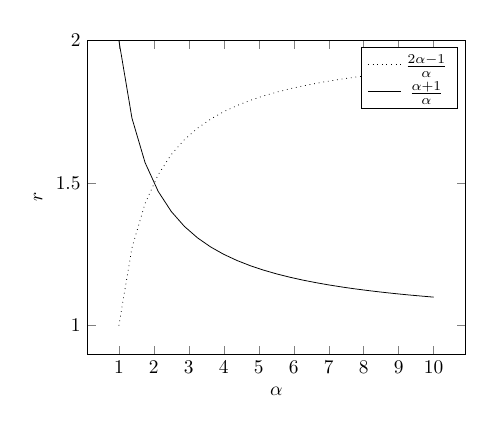
\begin{tikzpicture}[scale=0.70]
	\begin{axis}[
		domain=1:10, 
		ymax=2,
		xlabel = $\alpha$,
		ylabel = $r$,
		ytick = {1, 1.5, 2},
		xtick = {1, 2, 3, 4, 5, 6, 7, 8, 9, 10}
	] 
		\addplot[dotted]{(2 * x - 1) / (2 * x - x)}; %
		\addplot[black]{(x + 1) / x}; %()
		\legend{
	  		$\frac{2 \alpha - 1}{\alpha}$,
	  		$\frac{\alpha + 1}{\alpha}$
  		}
	\end{axis}
	\end{tikzpicture}
	\vspace{-5pt}
\caption{An upper bound on the approximation ratio as a function of $\alpha$.}
\label{fig:upper_bound}
\end{figure}

We show that our analysis is tight even for colored trees, using the
instance depicted in Fig.~\ref{fig:tight}, 
which consists of a colored graph where the greedy algorithm might recolor
$\frac{3}{2}$ times more vertices than the optimal convex recoloring.
%
We note that one can simply duplicate the instance using new colors for
each copy in order to construct an arbitrary large graph with the same
approximation ratio.

\begin{figure}[t]
\centering

\begin{tikzpicture}

\node (1) at (-2,0) [colored node, red node] {1};
\node (2) at (2,0) [colored node, red node] {2};
\node (3) at (0,0) [colored node, blue node] {3};
\node (4) at (4,0) [colored node, blue node] {4};
\node (5) at (-3,1) [colored node, green node] {5};
\node (6) at (-3,-1) [colored node, green node] {6};
\node (7) at (-1,-1) [colored node, black node] {7};
\node (8) at (1,-1) [colored node, black node] {8};

\draw (3) -- (8);
\draw (1) -- (6);
\draw (7) -- (3);
\draw (3) -- (2);
\draw (2) -- (4);
\draw (1) -- (3);
\draw (5) -- (1);

\end{tikzpicture}
\caption{
Greedy might choose to color the path (1, 3, 2), 
then it must recolor one of the vertices \{5, 6\} 
and one of the vertices \{7, 8\}, 
a total of three recolored vertices, 
while an optimal recoloring can color two paths: (5, 1, 6) and (7, 3, 8), 
a total of two recolored vertices.}
\label{fig:tight}
\end{figure}
